\documentclass{../document}

\addbibresource{refs.bib}

\begin{document}
	\title
		[Caltech SURF Second Interim Report]
		{Iago Mendes\fnote{\tt imendes@caltech.edu, ibrazmen@oberlin.edu}}
		{Control of Physical Parameters in Binary Black Hole Initial Data}
  
  \section{Calculation of asymptotic quantities}
    Since the first interim report, my focus has primarily been on the calculation of asymptotic quantities. In the Arnowitt-Deser-Misner (ADM) formalism, the total linear momentum is defined as an infinite-surface integral:
    \begin{equation} \label{eq:Padm}
      P_\text{ADM}^i = \frac{1}{8\pi} \oint_{S_\infty} (K^{ij} - K \gamma^{ij}) \, dS_j,
    \end{equation}
    \cite{Serguei}, where $K^{ij}$ is the inverse extrinsic curvature, $K$ is the extrinsic curvature trace, and $\gamma^{ij}$ is the inverse spatial metric. Evaluating this integral numerically can many times be inaccurate as the domain outer boundary is often sparse at large distances. To address this, we can use Gauss' law to recast \eqref{eq:Padm} as an infinite-volume integral:
    \begin{equation} \label{eq:Padm-volume}
      P_\text{ADM}^i = \frac{1}{8\pi} \oint_{S_0} P^{ij} \, dS_j - \frac{1}{8\pi} \int_{V_\infty} G^i \, dV
    \end{equation}
    \cite{Serguei}, where $S_0$ is some finite surface over which we evaluate the surface integral. We choose $S_0$ to be the domain excision sphere(s). In \eqref{eq:Padm},
    \begin{align}
      P^{ij} &= \psi^{10} (K^{ij} - K \gamma^{ij}), \\
      G^{i} &= \bar\Gamma^i_{jk} P^{jk}
             + \bar\Gamma^j_{jk} P^{jk}
             - 2 \bar\gamma_{jk} P^{jk} \bar\gamma^{il} \partial_l(\ln\psi)
    \end{align}
    \cite{Serguei}, where $\psi$ is the conformal factor, $\bar\gamma^{ij}$ is the inverse conformal metric, and $\bar\Gamma^i_{jk}$ are the conformal Christoffel symbols.

    Likewise, the total ADM mass is defined as
    \begin{equation} \label{eq:Madm}
      M_{ADM}
      = \frac{1}{16\pi} \oint_{S_\infty}  \Big(
        \bar\gamma^{jk} \bar\Gamma^i_{jk}
        - \bar\gamma^{ij} \bar\Gamma_{j}
        - 8 \bar\gamma^{ij} \partial_j \psi
        \Big) \, d\bar{S}_i
    \end{equation}
    \cite{BaumgarteShapiro}, where $\bar\Gamma_{i} = \bar\Gamma^j_{ij}$. We can also use Gauss' law in \eqref{eq:Madm}, giving us
    \begin{equation} \label{eq:Madm-volume}
      \begin{aligned}
        M_{ADM}
        &= \frac{1}{16\pi} \oint_{S_0}  \Big(
          \bar\gamma^{jk} \bar\Gamma^i_{jk}
          - \bar\gamma^{ij} \bar\Gamma_{j}
          - 8 \bar\gamma^{ij} \partial_j \psi
          \Big) \, d\bar{S}_i \\
        &\quad + \frac{1}{16\pi} \int_{V_\infty} \Big(
          \bar\gamma^{jk} \partial_i \bar\Gamma^i_{jk}
          + \bar\Gamma^i_{jk} \partial_i \bar\gamma^{jk}
          - \bar\gamma^{ij} \partial_i \bar\Gamma_j
          - \bar\Gamma_j \partial_i \bar\gamma^{ij}
          - 8 \bar D^2 \psi \Big) dV.
      \end{aligned}
    \end{equation}
    From the Hamiltonian constraint, we know that
    \begin{equation}
      8 \bar D^2 \psi = \psi \bar R + \frac{2}{3} \psi^5 K^2 - \frac{1}{4} \psi^5 \frac{1}{\alpha^2} \Big[ (\bar L \beta)_{ij} - \bar u_{ij} \Big] \Big[ (\bar L \beta)^{ij} - \bar u^{ij} \Big],
    \end{equation}
    where $\bar R$ is the conformal Ricci scalar, $\alpha$ is the lapse, $\beta$ is the shift, $\bar L$ is the longitudinal operator, and $\bar u_{ij} = \partial_t \bar\gamma_{ij}$.

    Finally, we can calculate the center of mass as
    \begin{equation} \label{eq:CoM}
      C_\text{CoM}^i = \frac{3}{8 \pi M_\text{ADM}} \oint_{S_\infty} \psi^4 \bar n^i \bar n^j \, d\bar{S}_j,
    \end{equation}
    where $\bar n^i = x^i / \bar r$ with $\bar r = (\bar\gamma_{ij} x^i x^j)^{1/2}$ and inertial coordinates $x^i$. Transforming \eqref{eq:CoM} with Gauss' law, we have
    \begin{equation} \label{eq:CoM-volume}
      \begin{aligned}
        C_\text{CoM}^i
        &= \frac{3}{8 \pi M_\text{ADM}} \oint_{S_0} \psi^4 \bar n^i \bar n^j \, d\bar{S}_j \\
        &\quad + \frac{3}{8 \pi M_\text{ADM}} \int_{V_\infty} \Big( 4 \psi^3 \partial_j \psi \bar n^i \bar n^j - \psi^4 \partial_j \bar\gamma_{kl} \bar n^i \bar n^j \bar n^k \bar n^l \Big) \, dV.
      \end{aligned}
    \end{equation}

	\section{Convergence tests}
    To check the implementation of the integrals described in the previous section, many convergence tests were performed. The main unit test uses a semi-analytic solution of a boosted Schwarzschild black hole. Figures \ref{fig:boosted-schwarzschild-no-volume} and \ref{fig:boosted-schwarzschild-with-volume} show how the results converge for this solution as we increase resolution. Similarly, Figures \ref{fig:bbh-no-volume} and \ref{fig:bbh-with-volume} display convergence tests for Binary Black Hole (BBH) initial data. In all these figures, “ref” stands for the value at the highest resolution and $R$ is the outer boundary radius, which effectively represents “infinity” for these integrals.

    From these convergence tests, we can note a few points. The ADM linear momentum infinite-volume integral \eqref{eq:Padm-volume} seems to perform slightly better than the infinite-surface integral \eqref{eq:Padm} at low resolutions, but the residuals are larger at high resolutions in BBH initial data. As for the ADM mass integrals, the infinite-volume version \eqref{eq:Madm-volume} appears to be less accurate than the infinite-surface version \eqref{eq:Madm}. This could be due to the higher number of numerical derivatives in the integrands. Lastly, the center of mass infinite-volume integral \eqref{eq:CoM-volume} does not converge as expected in both cases, suggesting a possible error in its implementation. Its infinite-surface counterpart \eqref{eq:CoM} converges up to a saturation point, which seems to depend on $R$.

    Overall, these tests indicate that the integrals are generally implemented correctly, but further investigation and improvements are necessary.

    \begin{figure}
      \centering
      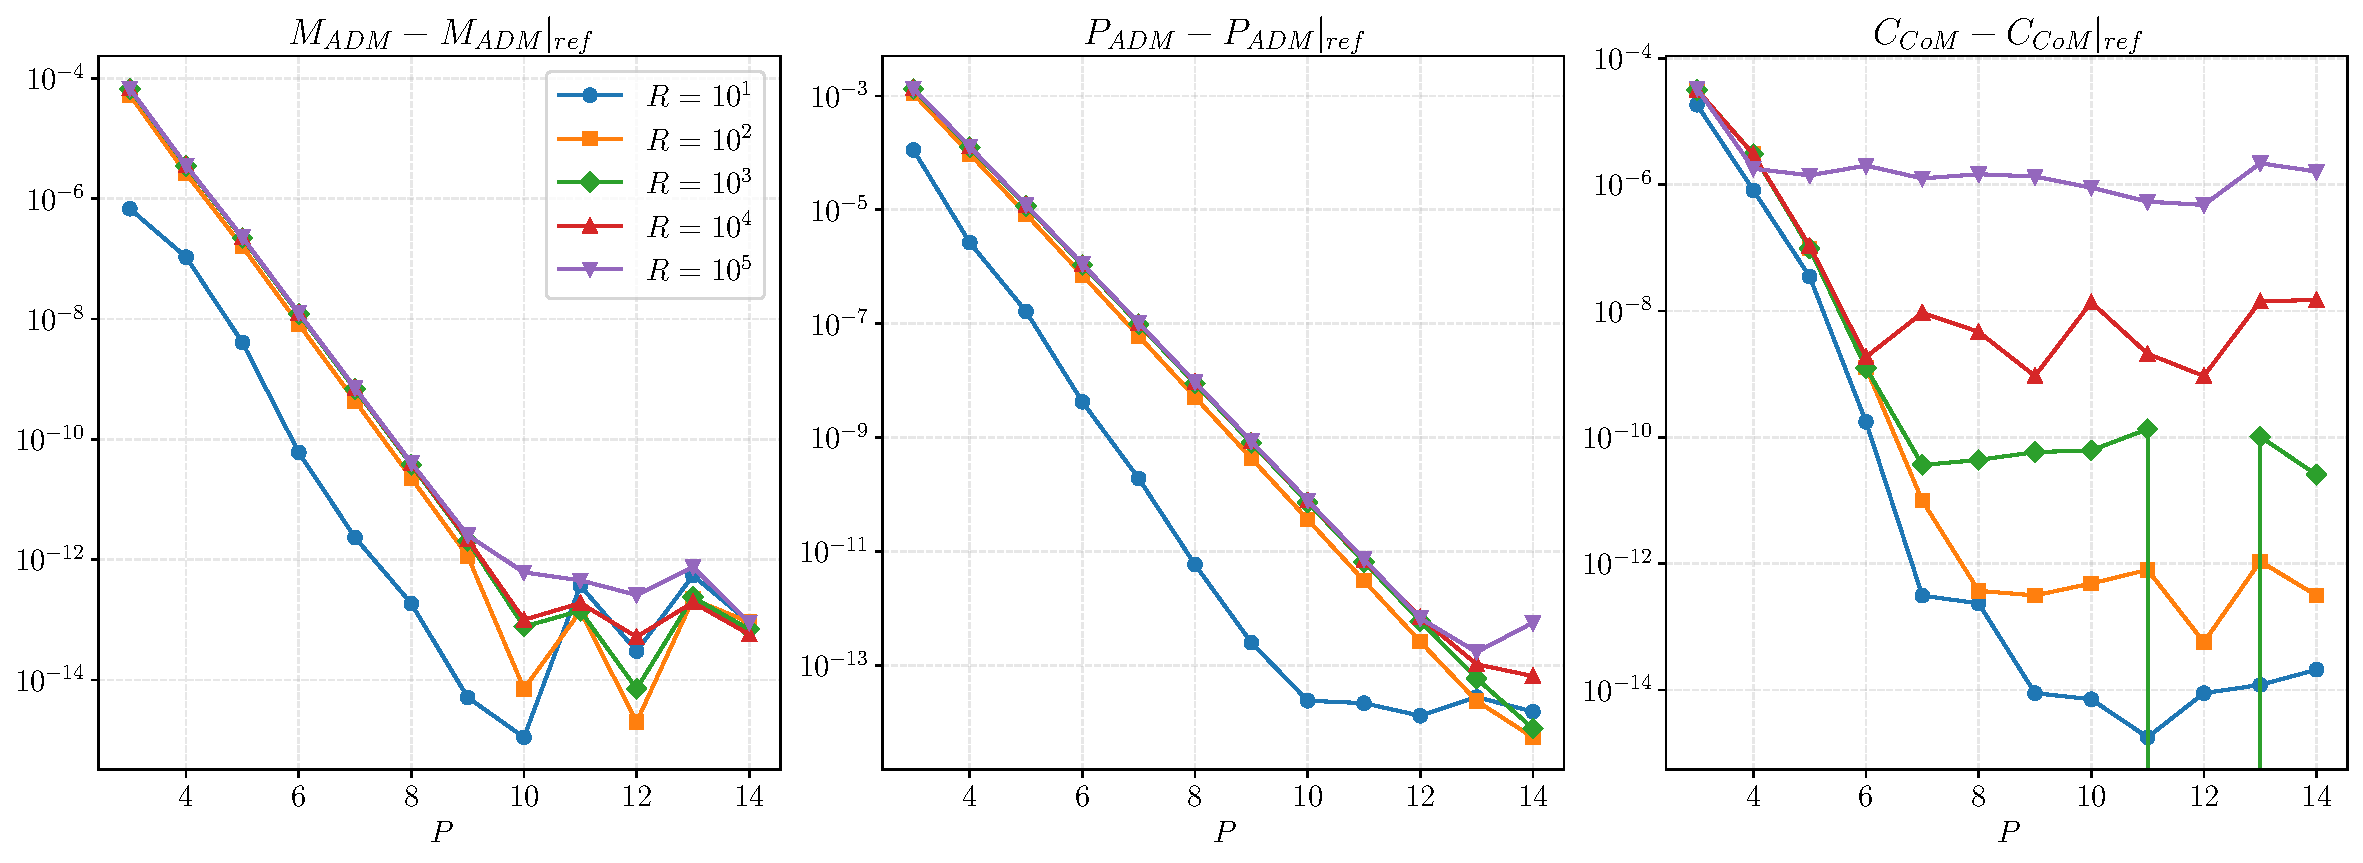
\includegraphics[width=0.95\textwidth]{assets/BoostedSchwarzschild_NoVolume.pdf}
      \caption{Convergence test of the infinite-surface integrals \eqref{eq:Madm}, \eqref{eq:Padm} and \eqref{eq:CoM} for a boosted Schwarzschild solution.}
      \label{fig:boosted-schwarzschild-no-volume}
    \end{figure}

    \begin{figure}
      \centering
      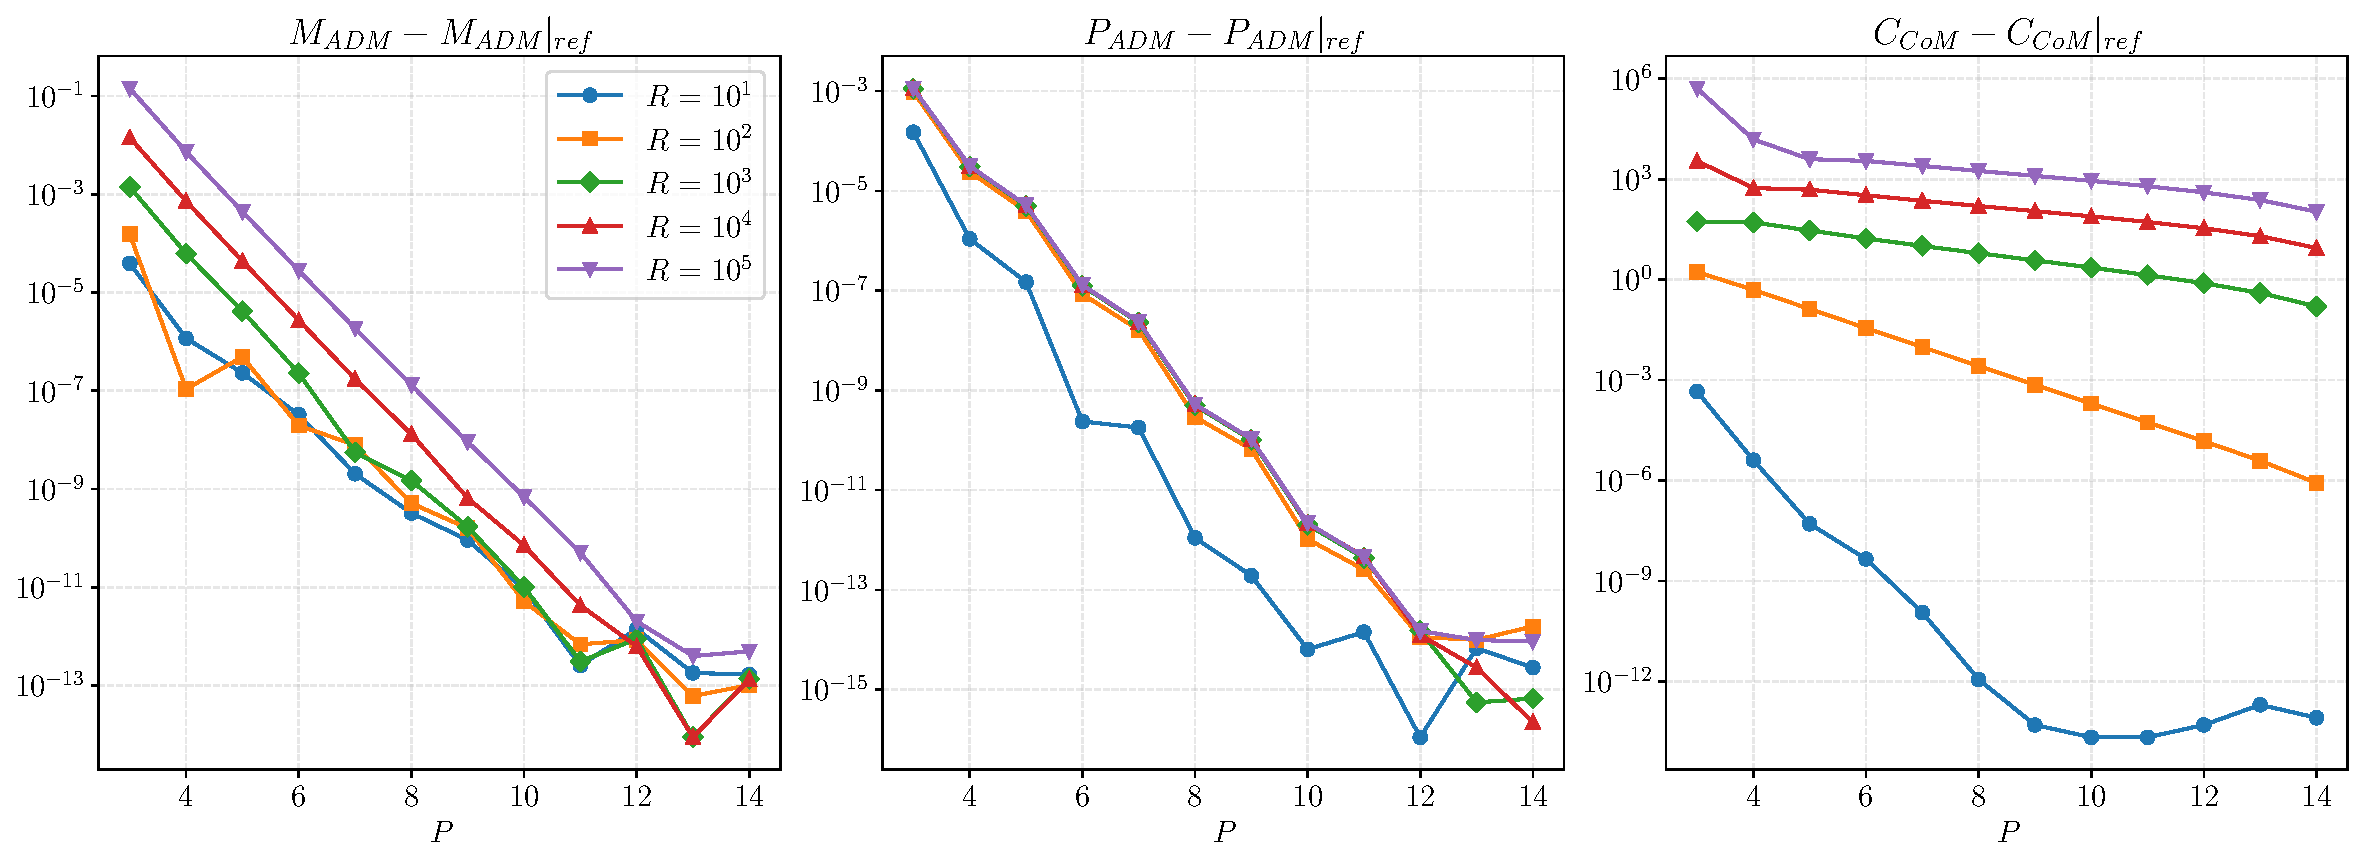
\includegraphics[width=0.95\textwidth]{assets/BoostedSchwarzschild_WithVolume.pdf}
      \caption{Convergence test of the infinite-volume integrals \eqref{eq:Madm-volume}, \eqref{eq:Padm-volume} and \eqref{eq:CoM-volume} for a boosted Schwarzschild solution.}
      \label{fig:boosted-schwarzschild-with-volume}
    \end{figure}

    \begin{figure}
      \centering
      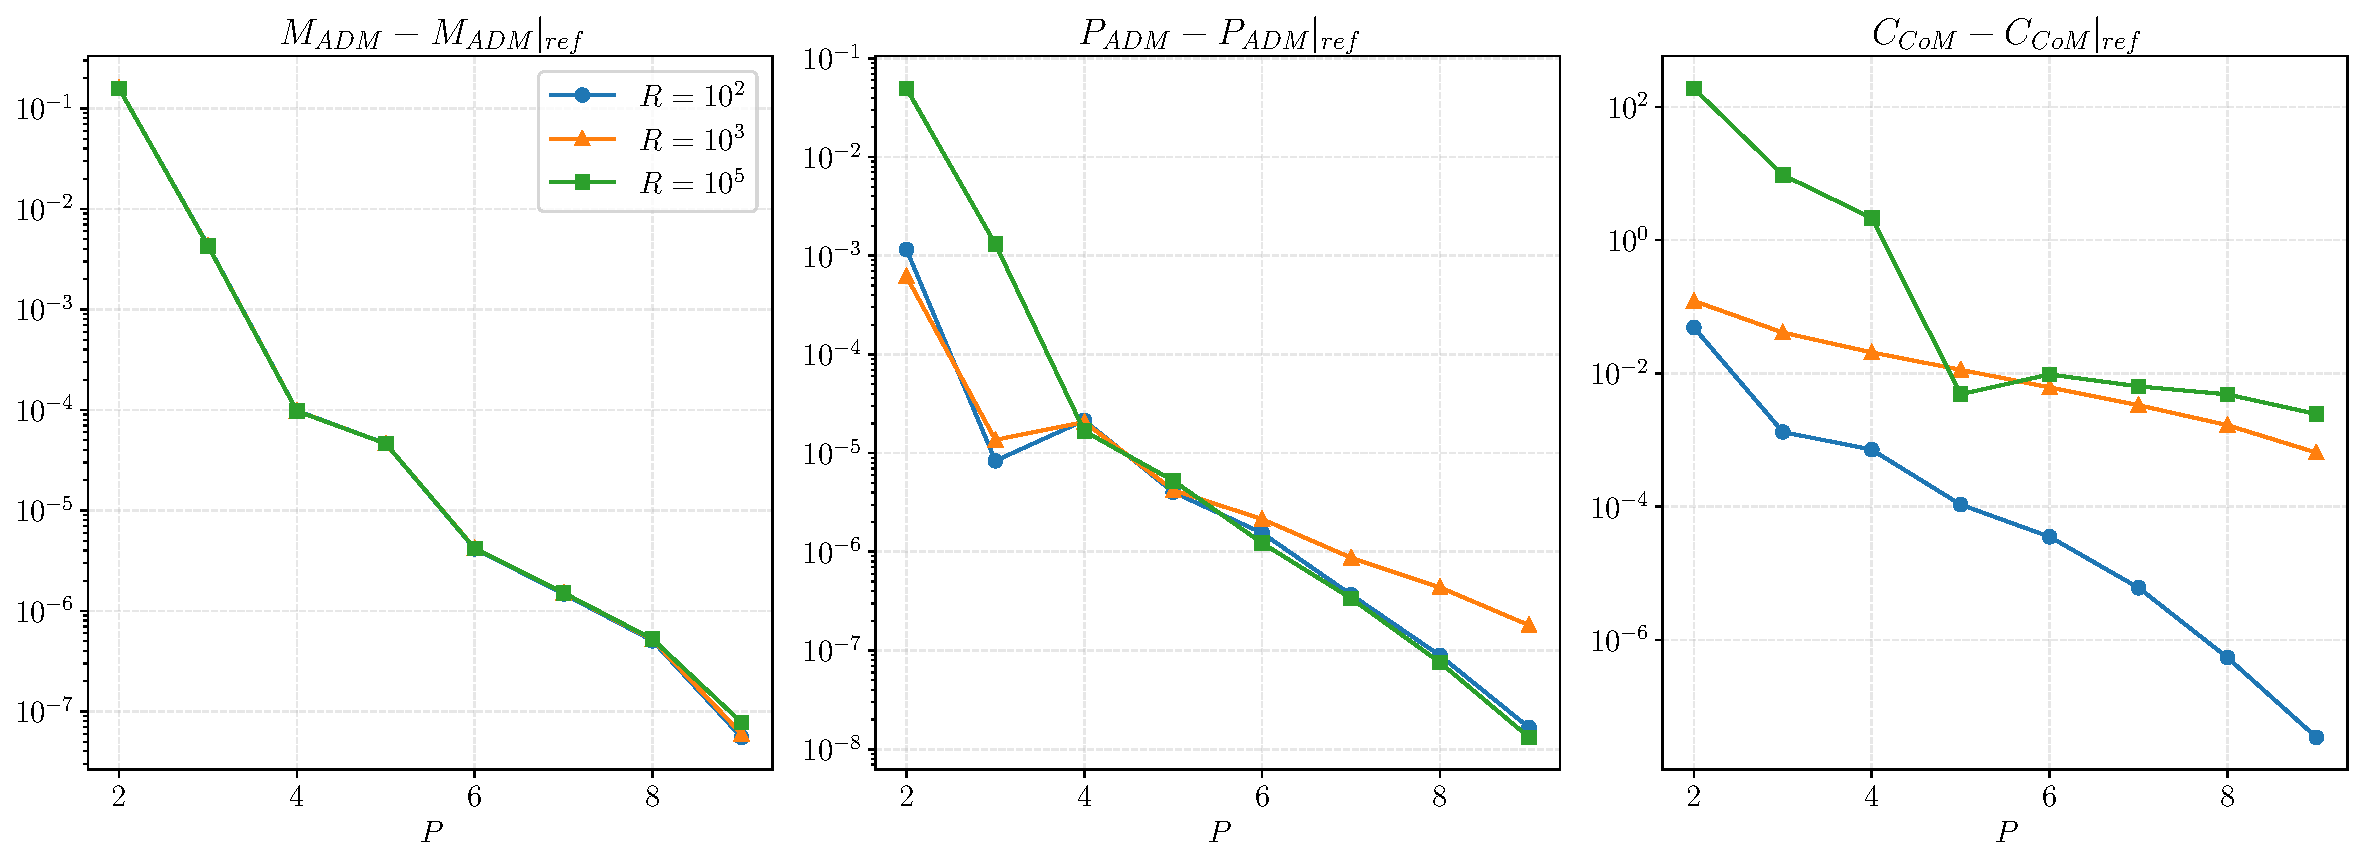
\includegraphics[width=0.95\textwidth]{assets/BBH_NoVolume.pdf}
      \caption{Convergence test of the infinite-surface integrals \eqref{eq:Madm}, \eqref{eq:Padm} and \eqref{eq:CoM} in a BBH initial data.}
      \label{fig:bbh-no-volume}
    \end{figure}

    \begin{figure}
      \centering
      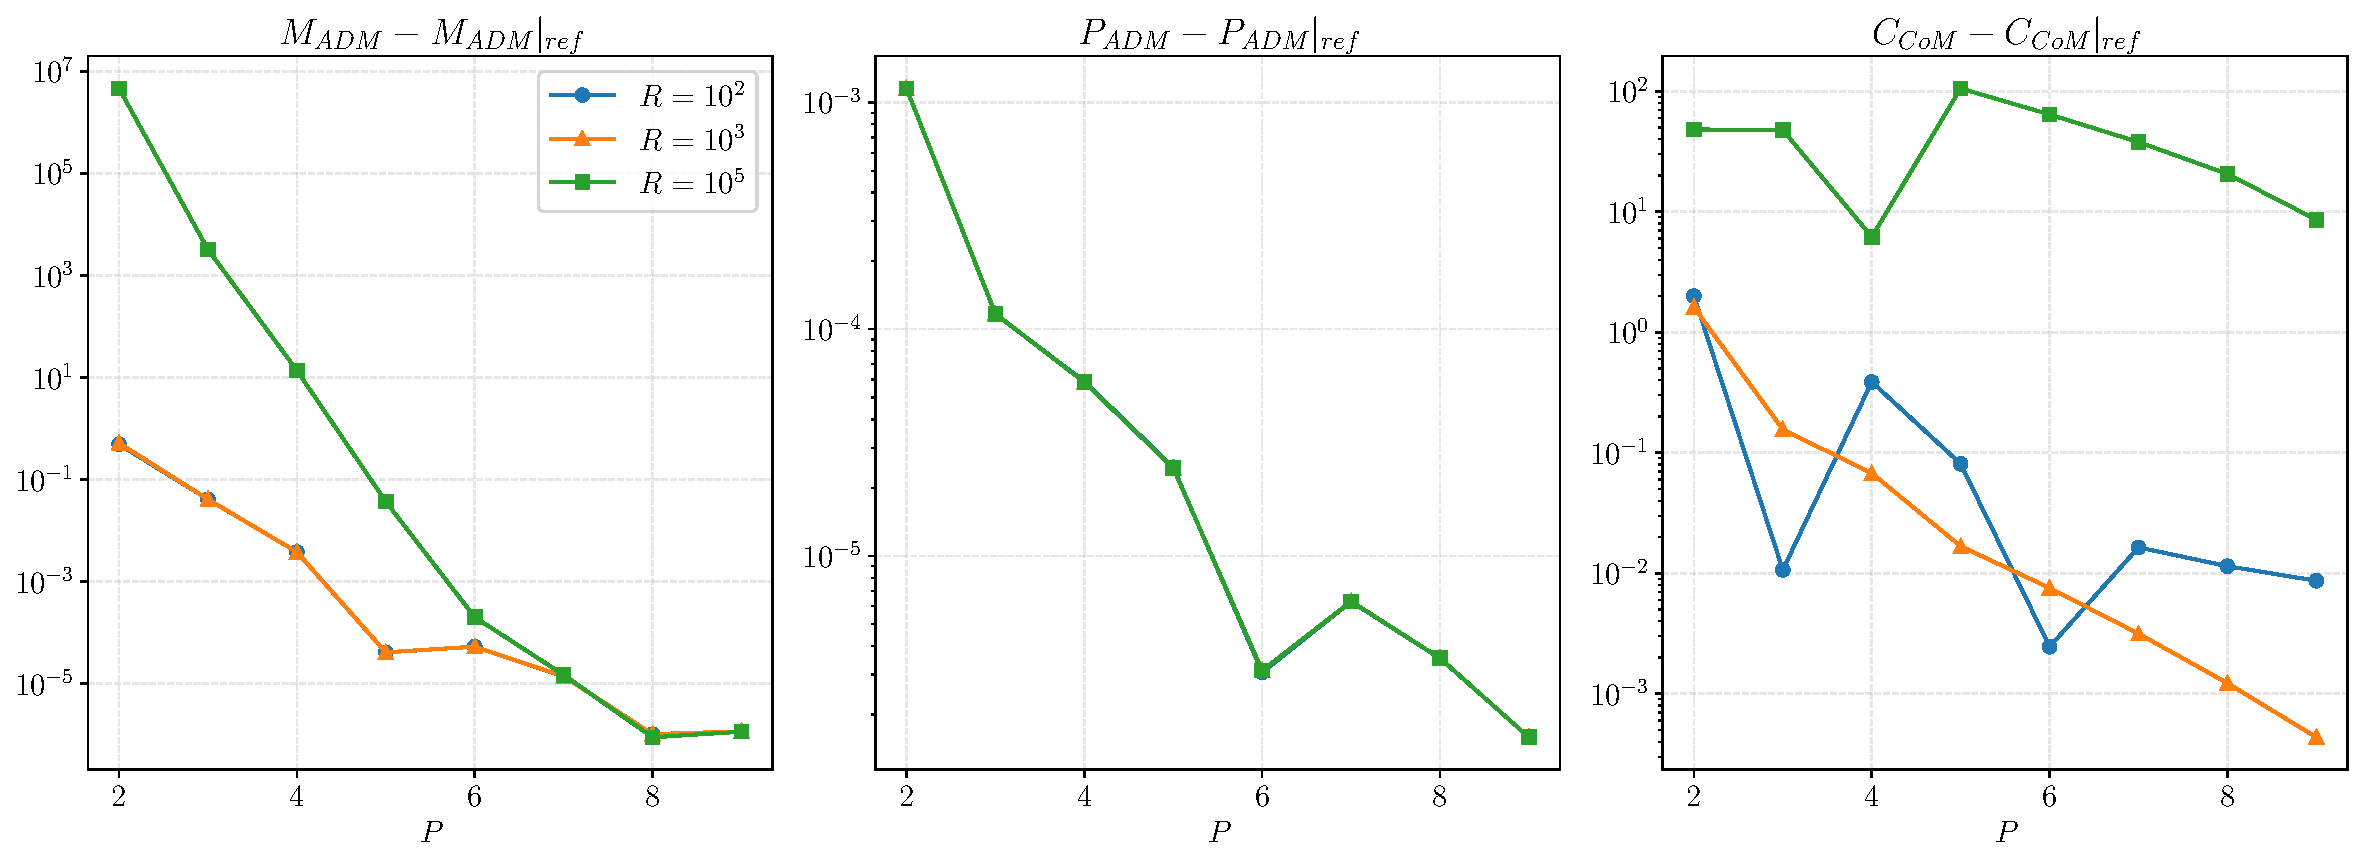
\includegraphics[width=0.95\textwidth]{assets/BBH_WithVolume.pdf}
      \caption{Convergence test of the infinite-volume integrals \eqref{eq:Madm-volume}, \eqref{eq:Padm-volume} and \eqref{eq:CoM-volume} in a BBH initial data.}
      \label{fig:bbh-with-volume}
    \end{figure}

	\section{Future Work}
    For the remainder of the project, my primary goal is to expand the iterative scheme from the first interim report to enable the control of center of mass and linear momentum. Given the current issues with the infinite-volume integrals, I plan to use the infinite-surface integrals until these issues are resolved. Additionally, I aim to implement the calculation of ADM angular momentum as defined in \cite{Serguei}, which may help clarify some of the problems we are encountering with the volume integrals. Being able to control the ADM angular momentum would also be useful for simulating hyperbolic encounters.

    Initially, I did not expect to allocate as much time to implementing the calculation of asymptotic quantities. My original plan included working on the control physical parameters after junk radiation has relaxed. However, I may not have sufficient time to address this aspect. If time permits, I would still like to explore modeling the effects of junk radiation on these physical parameters.

	\section*{References}
  	\printbibliography[heading=none]
\end{document}
